\documentclass[tikz,convert={outext=.svg,command=\unexpanded{pdf2svg \infile\space\outfile}},multi=false]{standalone}
\usepackage[utf8]{inputenc}

\usetikzlibrary{arrows,automata,shapes.geometric,decorations.pathmorphing,backgrounds,positioning,fit,petri, snakes}
\begin{document}


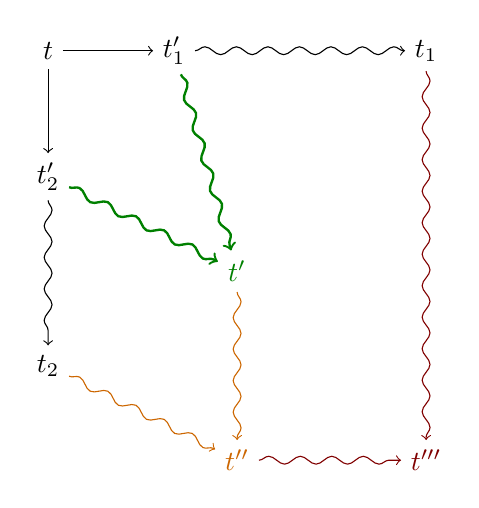
\begin{tikzpicture}[scale=0.8]
\tikzstyle{localconfluence}=[green!50!black, line width=0.3mm];
\tikzstyle{cloture}=[decorate, decoration={snake, segment length=4mm, amplitude=0.5mm}];
\tikzstyle{hyp1}=[orange!80!black];
\tikzstyle{hyp2}=[red!50!black];
\node (t) at (0, 0) {$t$};
\node (t1') at (2, 0) {$t_1'$};
\node (t1) at (6, 0) {$t_1$};
\node (t2') at (0, -2) {$t_2'$};
\node (t2) at (0, -5) {$t_2$};

\node[localconfluence] (t') at (3, -3.5) {$t'$};
\node[hyp1] (t'') at (3, -6.5) {$t''$};
\node[hyp2] (t''') at (6, -6.5) {$t'''$};


\draw[->] (t) edge (t1');
\draw[->] (t) edge (t2');

\draw[->, localconfluence] (t1') edge[cloture] (t');
\draw[->, localconfluence] (t2') edge[cloture] (t');

\draw[->, ] (t2') edge[cloture] (t2);
\draw[->, hyp1] (t') edge[cloture] (t'');
\draw[->, hyp1] (t2) edge[cloture] (t'');

\draw[->, ] (t1') edge[cloture] (t1);
\draw[->, hyp2] (t1) edge[cloture] (t''');
\draw[->, hyp2] (t'') edge[cloture] (t''');
\end{tikzpicture}

\end{document}